We begin by sketching the architecture of the SDN control plane and
illustrating the correctness challenges encountered by operators and
implementers.

SDN networks are managed by software running on a set of network-attached
servers called `controllers'. It is the job of the controllers to configure
the network in a way that complies with the intentions of network
operators. Operators codify their intentions by configuring
behavioral specifications we refer to as `policies'. Policy constraints
include connectivity, access control,
resource allocations, traffic engineering objectives, and middlebox
processing.

For fault-tolerance, production SDN control software is typically
distributed across multiple servers. For scalability, the responsibility for
managing the network can be partitioned through sharding.
Onix~\cite{onix}, for example, partitions a
graph of the network state across either an eventually consistent
distributed hash table or a
transactional database.
%allowing control applications to make their own
%tradeoffs in choosing consistency models and degree of fault tolerance.

In this distributed setting, controllers must coordinate amongst themselves
when reacting to state changes in the network or
policy changes from above.
Coordination in SDN is not exempt from the well-known class of faults
inherent to all distributed systems, such as
inconsistent reads, race conditions over message arrivals, and
unintended consequences of failover logic.

Several production SDN controllers support network
virtualization~\cite{bigswitch,nicirahomepage,contextream}, a technology that
abstracts the details of the underlying physical network and presents a
simplified view of the network to be configured by applications.
In this model, multi-tenancy is implemented by providing each tenant with their
own abstract network view, which are multiplexed onto the same physical network.
A common pattern is to treat an entire network as a single logical switch for each
tenant. When a large network is
abstracted in this way, the mapping between
the logical switch and the physical topology is highly complex.

In conjunction, the challenges of maintaining virtualized and distributed
objects while ensuring that critical invariants such as isolation between
tenants hold at all times make
SDN control software highly bug-prone.

To cope with these difficulties, software developers strive to thoroughly test
their software in a controlled environment before deploying to
production environments. The most common form of testing is unit testing,
where developers manually codify test cases to verify that individual software
components behave correctly. Each developer only has time to test a limited
number of cases though, and the number of test cases to consider is
practically unbounded, especially in
distributed systems. For this reason both of the SDN controller vendors we are
in contact with~\cite{nicirahomepage,bigswitch} employ a team of QA
engineers to automatically fuzz test their controller software on a testbed of switches and hosts.
When a bug is discovered in the QA testbed, it is first triaged
by a human, then logs are collected and sent to a developer for further troubleshooting.

Troubleshooting bugs found through QA testing is often an arduous task.
Fuzz tests frequently run for many hours before bugs are found, and involve
a large number of distributed nodes. Moreover, QA testing frameworks do little to mitigate
non-determinism, making it difficult for developers to replicate bugs.
Lastly, unlike the diverse set of tools available for debugging
individual programs, there are very few widely deployed debugging tools for
distributed systems~\cite{tooling_gap}; for highly non-deterministic bugs, it is not
uncommon for developers to throw
up their hands and simply wait until the next time the bug is observed before
continuing with diagnosis. It is our goal to improve this troubleshooting
process.

In the next section we give a formal definition of our approach to
troubleshooting. We then spend
the bulk of the paper describing how we realize this formalism.

% \subsection{Environment / Workflow}
\andi{maybe discuss in Section 2 what our expected environment / workflow is, so people know what
to expect. Do we position this as a developer tool? What's our input?}

%--------------------------------------------------------------------%
%               OLD HOTNETS TEXT
\eat{

% Peter: useful to state your assumptions:
%is correct: policies, logical layer specification, physical layer model
%is possibly buggy: logical -> physical layer

We begin by sketching the architecture of SDN networks and
describing the failure-modes and correctness challenges encountered by operators and
implementers of SDN control platforms.

SDN networks are managed by software running on a set of network-attached
servers called ``controllers''. Modern SDN platforms differ from
`first-generation' controllers such as NOX~\cite{nox} in two aspects: they
maintain a virtualized view on top of which control
logic resides, and they distribute state across
multiple control servers.

%Two common patterns of control are proactive and
%reactive. Proactive controllers pre-compute forwarding tables for the entire
%network, and only push down updates periodically to react to link failures,
%changes in traffic mix, \etc. In contrast, in \emph{reactive} SDNs, the
%controller updates the forwarding state in reaction to a \emph{dataplane event},
%e.g., a previously unmatched patched found on the wire.

%Production SDN deployments are commonly proactive, primarily due to the large
%scale of datacenter networks and the current capabilities of forwarding
%hardware. We focus on proactive controllers for the remainder of this paper,
%although our troubleshooting mechanisms are also applicable to reactive
%applications.

\subsection{Virtualization Challenges}

\colin{Reviewer OA: might be interpreted as tied to a specific SDN platform.}

\colin{Reviewer OD: does this architecture allow you to specify performance
policies?}

Modern SDN controllers consist of at least three distinct layers, as depicted in
Figure \ref{fig:basicarch}. The two lower layers are part of the SDN platform.
The lowest layer maintains a graph data-structure known as the \emph{physical view}
that has a one-to-one correspondence with the physical network.
Synchronization logic in this layer keeps its information up-to-date with the
physical network state. Above, the \emph{logical view} translates the
potentially complicated physical network to a simpler logical view, commonly a single
logical switch~\cite{Casado:2010:VNF:1921151.1921162}. If the control platform supports virtualization, a
virtualization layer handles multi-tenancy by providing each tenant with their
own logical view, which are multiplexed onto the same physical network.
Finally, at the top of the stack
the \emph{control application} specifies the desired
high-level behavior of the network by configuring the logical view. We term these behavioral specifications
``policies''. Policy constraints might include connectivity, access control,
addressing resource allocations, traffic engineering objectives, or middlebox
processing.

The logical view greatly simplifies the job of specifying policies. However, SDN
does not reduce the overall system complexity; it merely moves complexity out of
the control application and into the platform, which must transform these
high-level policy specifications into the appropriate configuration of each
physical device. When an entire datacenter network (up to 10,000 switches) is
abstracted into a single logical switch, the mapping between the logical switch
and the physical topology is highly complex.
%; for example, a simple configuration
%change such as ``the path from $A$ to $B$ should pass through $C$'' must be
%implemented as routing entries in a sequence of switches in the physical
%network.

\eat{
This mapping is further complicated in a multi-tenant environment
\cite{Casado:2010:VNF:1921151.1921162} where each tenant specifies policies on
their own logical switch. In such a case, each controller must deal with
multiple tenants, and each tenant's policies must be coordinated among multiple
controllers. Maintaining isolation between tenants is critical; updates to the
physical network must therefore be performed in a consistent fashion to ensure
that isolation breaches do not occur for any in-flight packets, despite hardware
failures and message delays.
}

\subsection{Distribution Challenges}

For fault-tolerance, production SDN control software is typically \emph{physically
distributed} on several control servers. For scalability, the responsibility for
managing the network can be partitioned through sharding between
several control servers. Onix~\cite{onix}, for example, partitions a
graph of the network state across either an eventually-consistent
distributed-hash table or a
transactional database, allowing control applications to make their own
tradeoffs in choosing consistency models and degree of fault tolerance.

Policy and state changes require coordination between controllers.
Coordination in SDN is not exempt from the well-known class of faults
inherent to all distributed systems, such as
inconsistent reads, race conditions over message arrivals, and
unintended consequences of failover logic.

In conjunction, the challenges of maintaining virtualized and distributed
objects while ensuring that critical invariants such as isolation between
tenants are upheld at all times makes the task of constructing
SDN control software highly complex and error-prone. We aim to provide a
technique to ease the process of troubleshooting bugs encountered in this
task.

\colin{Reviewer OE: Before we introduce so much new mechanism for
debugging networks, I'd like to see an analysis of the incidence of
these corner cases.}

\eat{
The large scale of these networks also means that
error events such as link failures or software crashes are common. Microsoft,
for example, reports 36M error events over one year across 8 datacenters, which
implies 8.5 error events per minute per
datacenter~\cite{Greenberg:2009:VSF:1592568.1592576}. 
}

\begin{figure}[t]
    %\hspace{-10pt}
    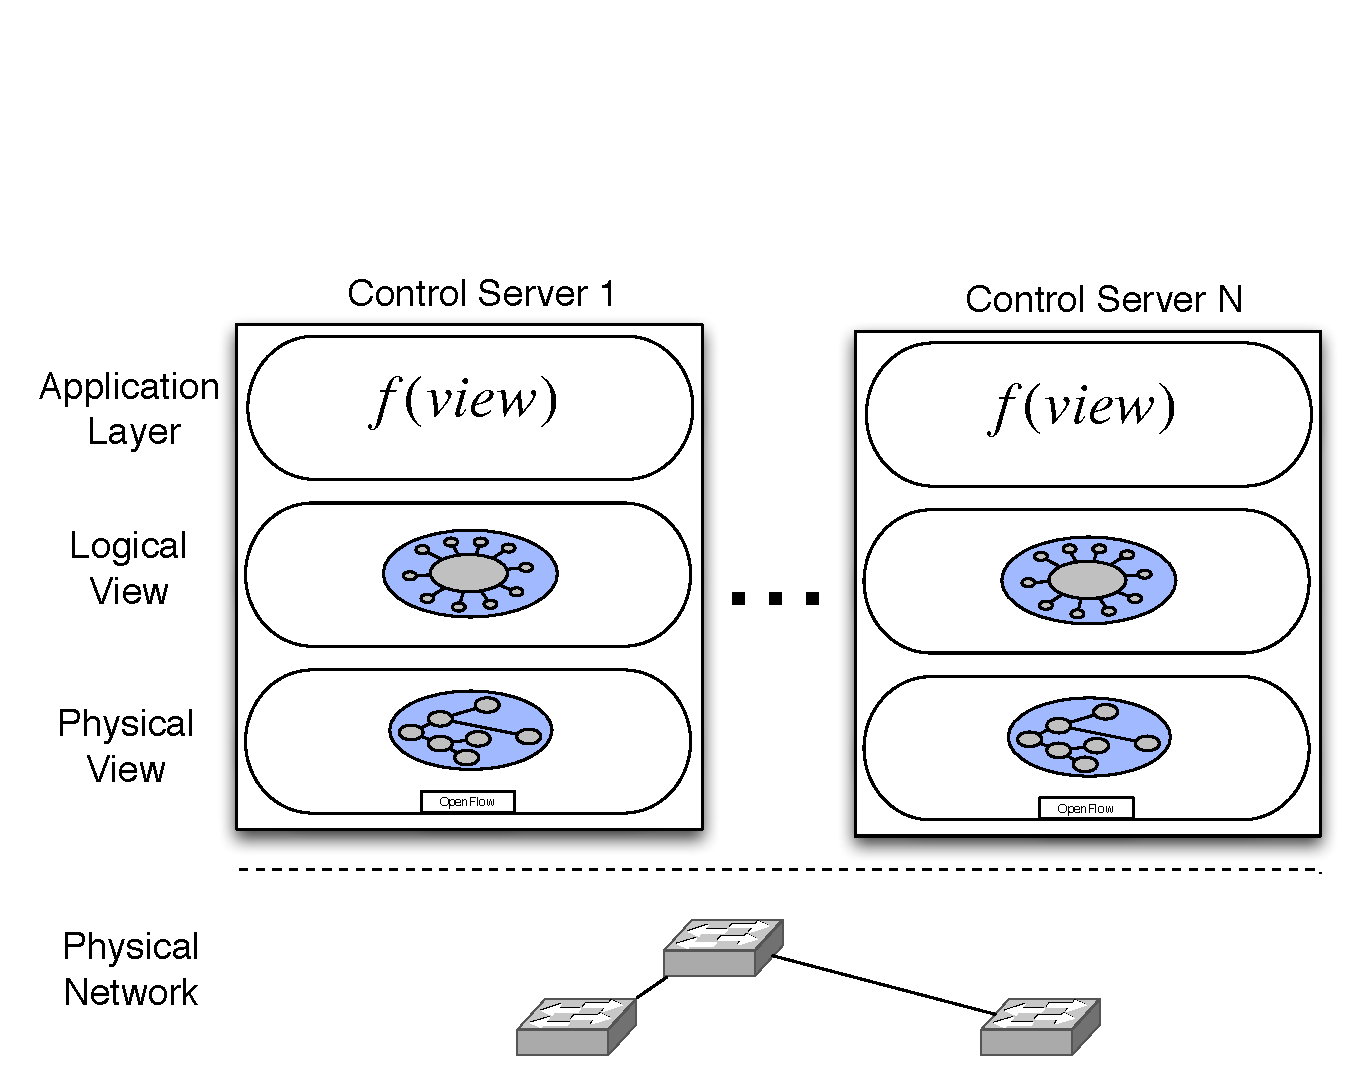
\includegraphics[width=3.25in]{../diagrams/architecture/SDN_Stack.pdf}
    \caption[]{\label{fig:basicarch} The SDN Software Architecture }
\end{figure}

\eat{
In this paper we focus on bugs in the virtualization and controller coordination
components of the SDN software stack. We focus on a \emph{proactive} mode of
operation where forwarding state updates are triggered by policy or topology
changes, not data-plane events.\footnote{It is possible to generalize our
approach to include inputs from the data-plane, subject to performance limitations.}
}

%We are primarily concerned with corner-case scenarios such as
%correlated hardware failures, which are the hardest to test {\it a priori}
%\andi{Check with our assumptions, i.e., uncorrelated external events}.
%Corner-case scenarios, while rare, cannot be ignored because of the distributed
%nature and large scale of production networks.
}
